\documentclass[twoside]{book}

% Packages required by doxygen
\usepackage{calc}
\usepackage{doxygen}
\usepackage{graphicx}
\usepackage[utf8]{inputenc}
\usepackage{makeidx}
\usepackage{multicol}
\usepackage{multirow}
\usepackage{textcomp}
\usepackage[table]{xcolor}

% NLS support packages
\usepackage[french]{babel}

% Font selection
\usepackage[T1]{fontenc}
\usepackage{mathptmx}
\usepackage[scaled=.90]{helvet}
\usepackage{courier}
\usepackage{amssymb}
\usepackage{sectsty}
\renewcommand{\familydefault}{\sfdefault}
\allsectionsfont{%
  \fontseries{bc}\selectfont%
  \color{darkgray}%
}
\renewcommand{\DoxyLabelFont}{%
  \fontseries{bc}\selectfont%
  \color{darkgray}%
}

% Page & text layout
\usepackage{geometry}
\geometry{%
  a4paper,%
  top=2.5cm,%
  bottom=2.5cm,%
  left=2.5cm,%
  right=2.5cm%
}
\tolerance=750
\hfuzz=15pt
\hbadness=750
\setlength{\emergencystretch}{15pt}
\setlength{\parindent}{0cm}
\setlength{\parskip}{0.2cm}
\makeatletter
\renewcommand{\paragraph}{%
  \@startsection{paragraph}{4}{0ex}{-1.0ex}{1.0ex}{%
    \normalfont\normalsize\bfseries\SS@parafont%
  }%
}
\renewcommand{\subparagraph}{%
  \@startsection{subparagraph}{5}{0ex}{-1.0ex}{1.0ex}{%
    \normalfont\normalsize\bfseries\SS@subparafont%
  }%
}
\makeatother

% Headers & footers
\usepackage{fancyhdr}
\pagestyle{fancyplain}
\fancyhead[LE]{\fancyplain{}{\bfseries\thepage}}
\fancyhead[CE]{\fancyplain{}{}}
\fancyhead[RE]{\fancyplain{}{\bfseries\leftmark}}
\fancyhead[LO]{\fancyplain{}{\bfseries\rightmark}}
\fancyhead[CO]{\fancyplain{}{}}
\fancyhead[RO]{\fancyplain{}{\bfseries\thepage}}
\fancyfoot[LE]{\fancyplain{}{}}
\fancyfoot[CE]{\fancyplain{}{}}
\fancyfoot[RE]{\fancyplain{}{\bfseries\scriptsize Généré le Samedi Novembre 21 2020 18\-:27\-:05 pour Pwd\-Pron\-Gen par Doxygen }}
\fancyfoot[LO]{\fancyplain{}{\bfseries\scriptsize Généré le Samedi Novembre 21 2020 18\-:27\-:05 pour Pwd\-Pron\-Gen par Doxygen }}
\fancyfoot[CO]{\fancyplain{}{}}
\fancyfoot[RO]{\fancyplain{}{}}
\renewcommand{\footrulewidth}{0.4pt}
\renewcommand{\chaptermark}[1]{%
  \markboth{#1}{}%
}
\renewcommand{\sectionmark}[1]{%
  \markright{\thesection\ #1}%
}

% Indices & bibliography
\usepackage{natbib}
\usepackage[titles]{tocloft}
\setcounter{tocdepth}{3}
\setcounter{secnumdepth}{5}
\makeindex

% Hyperlinks (required, but should be loaded last)
\usepackage{ifpdf}
\ifpdf
  \usepackage[pdftex,pagebackref=true]{hyperref}
\else
  \usepackage[ps2pdf,pagebackref=true]{hyperref}
\fi
\hypersetup{%
  colorlinks=true,%
  linkcolor=blue,%
  citecolor=blue,%
  unicode%
}

% Custom commands
\newcommand{\clearemptydoublepage}{%
  \newpage{\pagestyle{empty}\cleardoublepage}%
}


%===== C O N T E N T S =====

\begin{document}

% Titlepage & ToC
\hypersetup{pageanchor=false}
\pagenumbering{roman}
\begin{titlepage}
\vspace*{7cm}
\begin{center}%
{\Large Pwd\-Pron\-Gen }\\
\vspace*{1cm}
{\large Généré par Doxygen 1.8.5}\\
\vspace*{0.5cm}
{\small Samedi Novembre 21 2020 18:27:05}\\
\end{center}
\end{titlepage}
\clearemptydoublepage
\tableofcontents
\clearemptydoublepage
\pagenumbering{arabic}
\hypersetup{pageanchor=true}

%--- Begin generated contents ---
\chapter{Index des classes}
\section{Liste des classes}
Liste des classes, structures, unions et interfaces avec une brève description \-:\begin{DoxyCompactList}
\item\contentsline{section}{\hyperlink{class_password}{Password} \\*Classe représentant le mot de passe }{\pageref{class_password}}{}
\end{DoxyCompactList}

\chapter{Index des fichiers}
\section{Liste des fichiers}
Liste de tous les fichiers documentés avec une brève description \-:\begin{DoxyCompactList}
\item\contentsline{section}{\hyperlink{_password_8h}{Password.\-h} \\*Générateur de mot de passe prononçable }{\pageref{_password_8h}}{}
\end{DoxyCompactList}

\chapter{Documentation des classes}
\hypertarget{class_password}{\section{Référence de la classe Password}
\label{class_password}\index{Password@{Password}}
}


Classe représentant le mot de passe.  




{\ttfamily \#include \char`\"{}Définition\char`\"{}}

\subsection*{Fonctions membres publiques}
\begin{DoxyCompactItemize}
\item 
\hyperlink{class_password_a9ed0401599b14d501a8f46779048cdf2}{Password} ()
\begin{DoxyCompactList}\small\item\em Constructeur. \end{DoxyCompactList}\item 
virtual \hyperlink{class_password_ae019a63cb7332cb1c4e41d8ab7b4a619}{$\sim$\-Password} ()
\begin{DoxyCompactList}\small\item\em Destructeur. \end{DoxyCompactList}\item 
std\-::string \hyperlink{class_password_ab87e0e815c9193040046a3d945a3dbd3}{create\-Base\-Pwd} ()
\begin{DoxyCompactList}\small\item\em Création d'un mot de passe prononçable. \end{DoxyCompactList}\item 
std\-::string \hyperlink{class_password_a17cc4a113a56ec3dfc8b067e5d8805b0}{generate\-Pwd} (int length)
\begin{DoxyCompactList}\small\item\em Génération d'un mot de passe d'une longueur donnée. \end{DoxyCompactList}\end{DoxyCompactItemize}


\subsection{Description détaillée}
Classe représentant le mot de passe. 

La classe gère la génération d'un mot de passe 

\subsection{Documentation des constructeurs et destructeur}
\hypertarget{class_password_a9ed0401599b14d501a8f46779048cdf2}{\index{Password@{Password}!Password@{Password}}
\index{Password@{Password}!Password@{Password}}
\subsubsection[{Password}]{\setlength{\rightskip}{0pt plus 5cm}Password\-::\-Password (
\begin{DoxyParamCaption}
{}
\end{DoxyParamCaption}
)}}\label{class_password_a9ed0401599b14d501a8f46779048cdf2}


Constructeur. 

Constructeur de la classe \hyperlink{class_password}{Password} \hypertarget{class_password_ae019a63cb7332cb1c4e41d8ab7b4a619}{\index{Password@{Password}!$\sim$\-Password@{$\sim$\-Password}}
\index{$\sim$\-Password@{$\sim$\-Password}!Password@{Password}}
\subsubsection[{$\sim$\-Password}]{\setlength{\rightskip}{0pt plus 5cm}Password\-::$\sim$\-Password (
\begin{DoxyParamCaption}
{}
\end{DoxyParamCaption}
)\hspace{0.3cm}{\ttfamily [virtual]}}}\label{class_password_ae019a63cb7332cb1c4e41d8ab7b4a619}


Destructeur. 

Destructeur de la classe \hyperlink{class_password}{Password}; 

\subsection{Documentation des fonctions membres}
\hypertarget{class_password_ab87e0e815c9193040046a3d945a3dbd3}{\index{Password@{Password}!create\-Base\-Pwd@{create\-Base\-Pwd}}
\index{create\-Base\-Pwd@{create\-Base\-Pwd}!Password@{Password}}
\subsubsection[{create\-Base\-Pwd}]{\setlength{\rightskip}{0pt plus 5cm}std\-::string Password\-::create\-Base\-Pwd (
\begin{DoxyParamCaption}
{}
\end{DoxyParamCaption}
)}}\label{class_password_ab87e0e815c9193040046a3d945a3dbd3}


Création d'un mot de passe prononçable. 

Méthode qui permet la création d'un mot de passe prononçable de 9 caractères composé ainsi\-:
\begin{DoxyItemize}
\item 2 séquences consonne-\/voyelle-\/consonne
\item 1 chiffre
\item 2 caractères spéciaux (.,?;\-:!\-\_\--\/()\mbox{[}\mbox{]}=\{\}\#+\&$\ast$\%\$$<$$>$)
\end{DoxyItemize}

A partir de la fonction P\-H\-P créée par Andreas Gohr et adaptée par Yannick Sebastia

\begin{DoxyReturn}{Renvoie}
mot de passe prononçable 
\end{DoxyReturn}
\hypertarget{class_password_a17cc4a113a56ec3dfc8b067e5d8805b0}{\index{Password@{Password}!generate\-Pwd@{generate\-Pwd}}
\index{generate\-Pwd@{generate\-Pwd}!Password@{Password}}
\subsubsection[{generate\-Pwd}]{\setlength{\rightskip}{0pt plus 5cm}std\-::string Password\-::generate\-Pwd (
\begin{DoxyParamCaption}
\item[{int}]{length}
\end{DoxyParamCaption}
)}}\label{class_password_a17cc4a113a56ec3dfc8b067e5d8805b0}


Génération d'un mot de passe d'une longueur donnée. 

Méthode pour générer un mot de passe supérieur à 9 caractères.


\begin{DoxyParams}{Paramètres}
{\em length} & \-: longueur du mot de passe \\
\hline
\end{DoxyParams}
\begin{DoxyReturn}{Renvoie}
mot de passe prononçable de longueur {\itshape length} 
\end{DoxyReturn}


La documentation de cette classe a été générée à partir des fichiers suivants \-:\begin{DoxyCompactItemize}
\item 
\hyperlink{_password_8h}{Password.\-h}\item 
Password.\-cpp\end{DoxyCompactItemize}

\chapter{Documentation des fichiers}
\hypertarget{_password_8h}{\section{Référence du fichier Password.\-h}
\label{_password_8h}\index{Password.\-h@{Password.\-h}}
}


Générateur de mot de passe prononçable.  


{\ttfamily \#include $<$string$>$}\\*
{\ttfamily \#include $<$iostream$>$}\\*
{\ttfamily \#include $<$ctime$>$}\\*
{\ttfamily \#include $<$cstdlib$>$}\\*
Graphe des dépendances par inclusion de Password.\-h\-:
\nopagebreak
\begin{figure}[H]
\begin{center}
\leavevmode
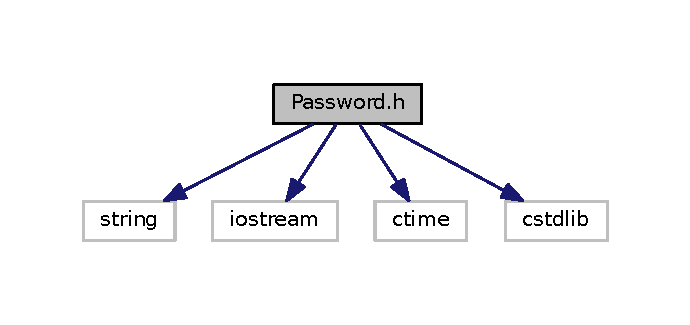
\includegraphics[width=331pt]{_password_8h__incl}
\end{center}
\end{figure}
\subsection*{Classes}
\begin{DoxyCompactItemize}
\item 
class \hyperlink{class_password}{Password}
\begin{DoxyCompactList}\small\item\em Classe représentant le mot de passe. \end{DoxyCompactList}\end{DoxyCompactItemize}


\subsection{Description détaillée}
Générateur de mot de passe prononçable. \begin{DoxyAuthor}{Auteur}
jn-\/glx 
\end{DoxyAuthor}
\begin{DoxyDate}{Date}
21 nov. 2020 
\end{DoxyDate}
\begin{DoxyVersion}{Version}
0.\-1 
\end{DoxyVersion}

%--- End generated contents ---

% Index
\newpage
\phantomsection
\addcontentsline{toc}{part}{Index}
\printindex

\end{document}
